\documentclass[border=4pt]{standalone}
\usepackage{tikz}
\usetikzlibrary{positioning, arrows.meta, calc, fit, backgrounds}
\usepackage{amsmath,amssymb}

\begin{document}
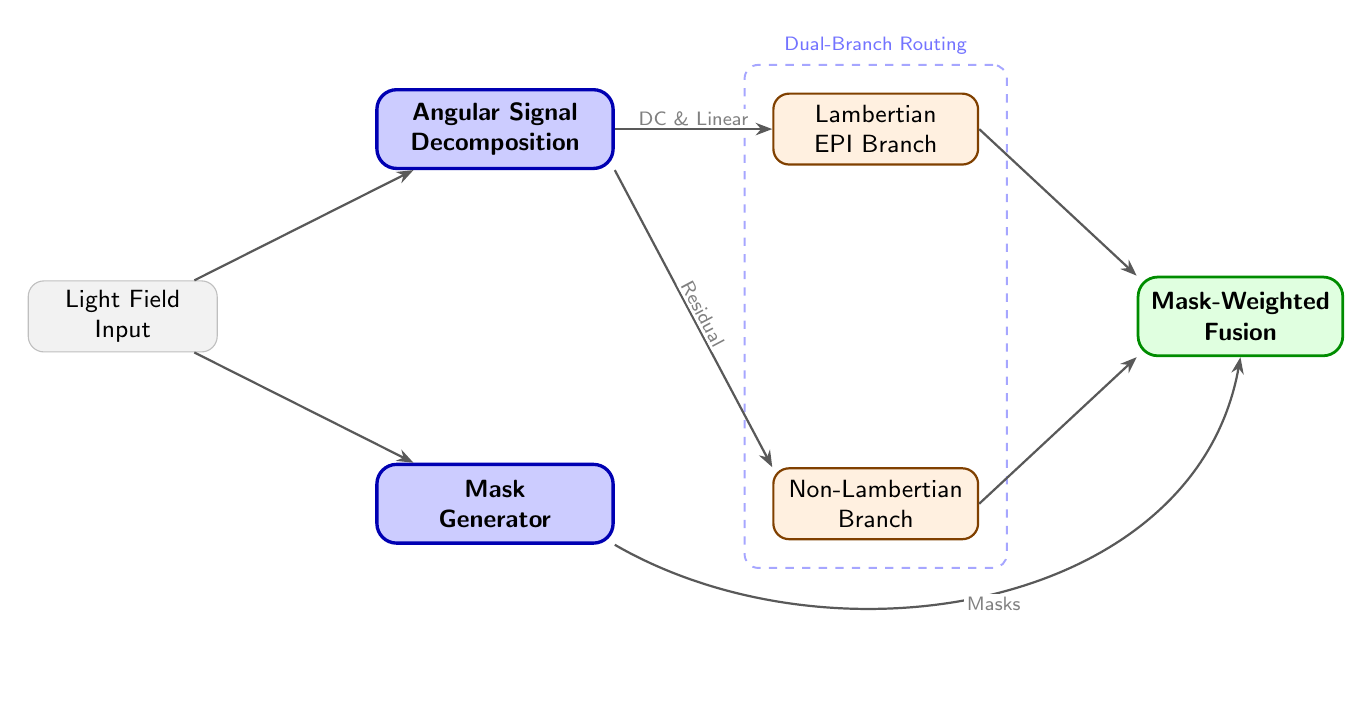
\begin{tikzpicture}[
  input/.style={draw, rounded corners=2mm, minimum width=2.4cm, minimum height=0.9cm,
                fill=gray!10, draw=gray!50, align=center, font=\sffamily\small},
  innov/.style={draw, rounded corners=2.5mm, minimum width=3cm, minimum height=1cm,
                fill=blue!20, draw=blue!70!black, line width=1.2pt, align=center,
                font=\sffamily\small\bfseries},
  branch/.style={draw, rounded corners=2mm, minimum width=2.6cm, minimum height=0.9cm,
                 fill=orange!12, draw=orange!50!black, line width=0.8pt, align=center,
                 font=\sffamily\small},
  output/.style={draw, rounded corners=2.5mm, minimum width=2.6cm, minimum height=1cm,
                 fill=green!12, draw=green!55!black, line width=1pt, align=center,
                 font=\sffamily\small\bfseries},
  arr/.style={-{Stealth[length=6pt]}, thick, color=black!65},
  lbl/.style={font=\sffamily\scriptsize, text=black!50, fill=white, inner sep=1pt},
  gbox/.style={draw=blue!35, dashed, rounded corners=5pt, inner sep=10pt, line width=0.7pt},
]

% Input
\node[input] (m1) {Light Field\\Input};

% Core innovations (column 2)
\node[innov, above right=1.4cm and 2cm of m1] (m2)
  {\textbf{Angular Signal}\\\textbf{Decomposition}};
\node[innov, below right=1.4cm and 2cm of m1] (m3)
  {\textbf{Mask}\\\textbf{Generator}};

% Dual branches (column 3)
\node[branch, right=2cm of m2] (m4) {Lambertian\\EPI Branch};
\node[branch, right=2cm of m3] (m5) {Non-Lambertian\\Branch};

% Output — compute merge midpoint
\path (m4.east) -- (m5.east) coordinate[midway] (midmerge);
\node[output, right=2cm of midmerge] (m6)
  {\textbf{Mask-Weighted}\\\textbf{Fusion}};

% === Arrows (main flow) ===
\draw[arr] (m1) -- (m2);
\draw[arr] (m1) -- (m3);

\draw[arr] (m2) -- node[lbl, above] {DC \& Linear} (m4);
\draw[arr] (m2.south east) -- node[lbl, above, sloped] {Residual} (m5.north west);

% Route m3 -> m6 below m5 to avoid crossing
\draw[arr] (m3.south east) to[out=-30, in=-100]
  node[lbl, below, pos=0.5] {Masks} (m6.south);

\draw[arr] (m4.east) -- (m6.north west);
\draw[arr] (m5.east) -- (m6.south west);

% Dual-branch routing group box
\begin{scope}[on background layer]
  \node[gbox, fit=(m4)(m5),
        label={[font=\sffamily\scriptsize, text=blue!55]above:Dual-Branch Routing}] {};
\end{scope}

\end{tikzpicture}
\end{document}